\fancyfoot[C]{G�rel}
\subsection{Kartographie Algorithmen}
In ROS stehen verschiedene Algorithmen zur Verf�gung, die es Robotern erm�glichen, ihre Umgebung zu kartieren und eine interne Darstellung der Welt um sie herum zu erstellen. Diese spielen eine entscheidende Rolle bei der Umgebungswahrnehmung und der sicheren Navigation von Robotern.

\paragraph{Hector SLAM}
Hector SLAM \cite{Kohlbrecher2011}ist ein Kartographie Algorithmus in ROS, der auf der Nutzung von Laserscannern basiert. Dieser Algorithmus verwendet eine Sch�tzmethode, um die Position und Orientierung eines Roboters basierend auf den Laserdaten zu bestimmen. Durch kontinuierliches Scannen der Umgebung und die Verfolgung von Merkmalen kann Hector SLAM eine pr�zise Karte der Umgebung erstellen. Ein wesentlicher Vorteil dieses Algorithmus ist seine Effizienz und Robustheit, auch in Umgebungen mit begrenzter Sichtbarkeit oder Bewegungseinschr�nkungen.

\paragraph{Google Cartographer}
Google Cartographer \cite{Hess2016}, ein in ROS integrierter Kartographie Algorithmus, basiert auf dem Prinzip der simultanen Lokalisierung und Kartierung (SLAM), wobei er Laserscanner- und IMU-Daten nutzt, um eine Karte der Umgebung zu generieren. Google Cartographer wird h�ufig in autonomen Fahrzeugen und Robotern eingesetzt, um pr�zise Umgebungskarten zu erstellen. Eine besonders herausragende Eigenschaft des Google Cartographers liegt in seiner Unabh�ngigkeit von Odometriedaten, was ihn besonders attraktiv macht, insbesondere bei diesem Projekt, da solche Daten nicht vollst�ndig verf�gbar sind. Diese Option erweist sich als vorteilhaft und erm�glicht eine zuverl�ssige Kartierung auch unter herausfordernden Bedingungen.
\begin{figure}[H]
    \centering
    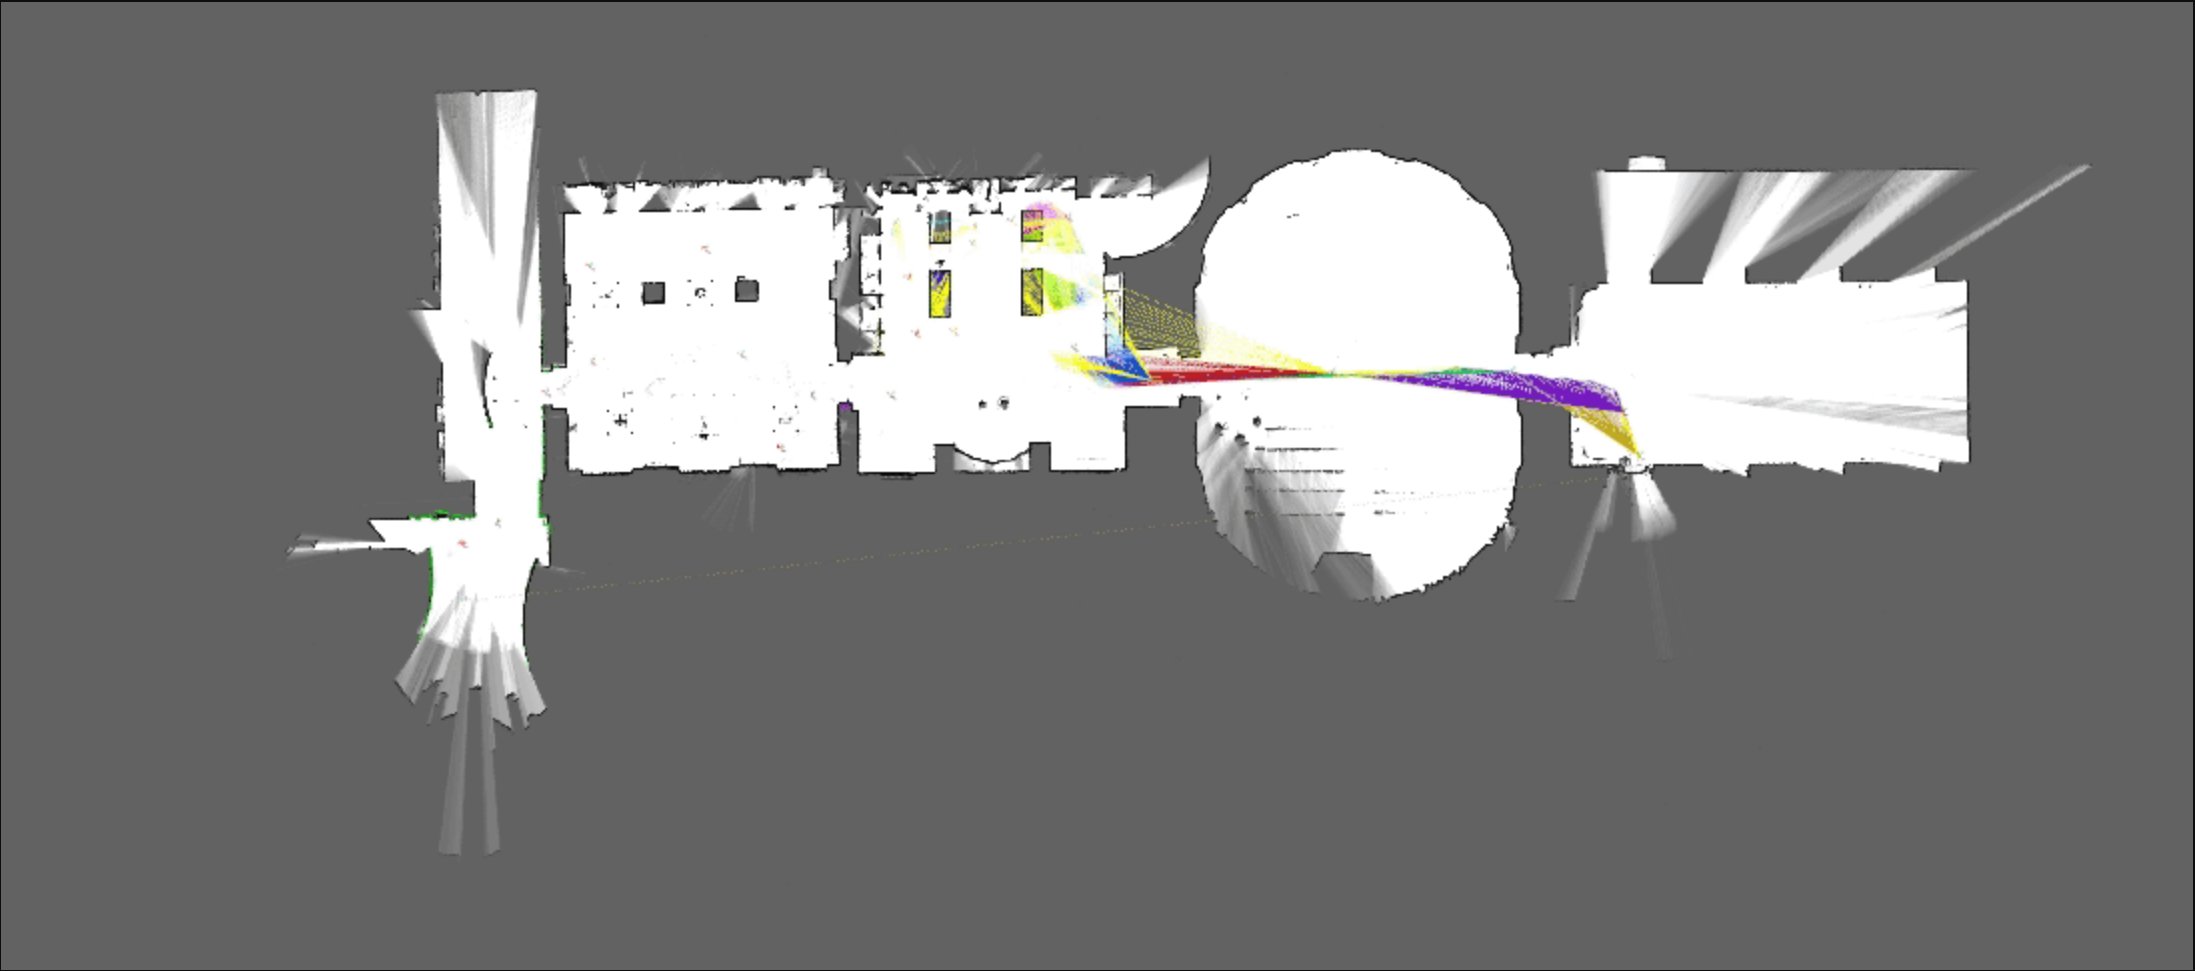
\includegraphics[scale=0.165]{./3_Stand_der_Technik/Abbildungen/google_slam_symbolbild.png}
    \caption{Symbolbild einer erstellten Karte vom Cartographer \cite{Hess2016}}
\end{figure}
\paragraph{Anpassung und Integration}
Beide Kartographie Algorithmen bieten M�glichkeiten zur Anpassung und Integration in ROS. Entwickler k�nnen die Parameter der Algorithmen an die spezifischen Anforderungen ihres Projekts anpassen und sie in bestehende Robotikanwendungen integrieren. Dies erm�glicht es, hochpr�zise Karten der Umgebung zu erstellen und sie f�r die Navigation und Steuerung von Robotern zu verwenden.
